 % PrivateMsg


  \subsection{Consumption Concavity}\label{sec:def_CC}
  We start by defining what we mean by consumption concavity (CC) and greater consumption concavity.

  \begin{defn}\label{defn:IntervalStrictCC} (Local Consumption Concavity.) \\ In relation to a
    utility function $u(c)$ with $u'>0$, $u''<0$, and non-negative ($u''' \geq 0$) and non-increasing prudence, a function $V({m})$ has property CC (alternately, strict CC) over the
    interval between ${m}_{1}$ and ${m}_{2}$, where ${m}_2 >{m}_{1}$, if
    \begin{equation*}
      V'({m}) = u'(c({m}))
\end{equation*}
    for some increasing function $c({m})$ that satisfies concavity (alternately, strict concavity) over the interval from ${m}_{1}$ to ${m}_{2}$.
  \end{defn}
  \noindent Since (even with constraints) $V'({m}) = u'(c({m}))$ holds by the envelope theorem, $V({m})$ having property CC (alternately, strict CC) is the same as having a concave (alternately, strictly concave) consumption function $c({m})$.\footnote{Remember that the envelope theorem depends only on being able to spend \textit{current} wealth on \textit{current} consumption, so it holds whether or not there is a 	liquidity constraint.} Note that the definition is restricted to non-negative and non-increasing prudence. This encompasses most of the commonly used utility functions in the economics literature (e.g.\ CRRA, CARA, quadratic). Also, note that we allow for `non-strict' concavity -- that is, linearity -- because we want to include cases such as quadratic utility in which parts of the consumption function can be linear.  Henceforth, unless otherwise noted, we will drop the cumbersome usage `alternately, strict' -- the reader should assume that what we mean always applies in the two alternate cases in parallel.

  If a function has property local CC at every point, we define it as having property CC globally.
  \begin{defn}\label{defn:PropCC} (Global Consumption Concavity.) \\  A function $V({m})$ has property CC in relation to a utility function $u(c)$ with $u'>0$, $u''<0$, and non-negative ($u''' \geq 0$) and non-increasing prudence if $V'({m}) = u'(c({m}))$ for some monotonically increasing concave function $c({m})$.
  \end{defn}

  \noindent We now show that once a value function exhibits the property CC in some period $t+1$, it will also have the property CC in period $t$ and earlier under fairly general conditions. Lemma \ref{lem:recursive} formally provides conditions guaranteeing this recursive propagation.

  \begin{lemma}\label{lem:recursive}(Recursive Propagation of Consumption Concavity.) \\
    Consider an agent with a HARA utility function satisfying $u' > 0$, $u'' < 0$, $u''' \geq 0$ and non-increasing absolute prudence ($-u'''/u''$). Assume that no liquidity constraint applies at the end of period $t$ and that the agent faces income risk $y_{t+1} \in [\underline{y},\bar{y}]$. If $V_{t+1}({m}_{t+1})$ exhibits property (local) CC for all ${m}_{t+1} \in [R{a}_{t} + \underline{y}, R{a}_{t} + \bar{y}]$, then $V_t({m}_{t})$ exhibits property (local) CC at the level of wealth ${m}_{t}$ such that optimal consumption yields ${a}_{t} = {m}_{t} - c_t({m}_{t})$.

    \medskip
    \noindent If also $V_{t+1}({m}_{t+1})$ exhibits property strict (local) CC for at least one ${m}_{t+1} \in [R{a}_{t} + \underline{y}, R{a}_{t} + \bar{y}]$, then $V_t({m}_{t})$ exhibits property strict (local) CC at the level of wealth ${m}_{t}$ where optimal consumption yields ${a}_{t} = {m}_{t} - c_t({m}_{t})$.
  \end{lemma}
  \noindent See Appendix \ref{app:recursive} for the proof. The basic insight of Lemma \ref{lem:recursive} is that as long as the future consumption function is concave for all realizations of $y_{t+1}$, then it is also concave today. Additionally, if the the future consumption function is strictly concave for at least one realization of ${y}_{t+1}$, then the consumption function is strictly concave also today.


  The last concept we define is when a value function exhibits `greater' concavity than another. This will allow us to compare two consumption functions and their respective concavity later.
  \begin{defn}\label{defn:MoreCC} (Greater Consumption Concavity.) \\ Consider two functions $V({m})$ and $\hat{V}({m})$ that both exhibit property CC with respect to the same $u(c)$ at a point ${m}$ for some interval $({m}_1,{m}_2)$ such that ${m}_1 < {m} < {m}_2$.  Then $\hat{V}({m})$ exhibits property `greater CC' compared to $V({m})$ if
    \begin{eqnarray}
      \hat{c}({m}) - \left(\frac{{m}_{2}-{m}}{{m}_{2}-{m}_{1}} \hat{c}({m}_{1})+\frac{{m}-{m}_{1}}{{m}_{2}-{m}_{1}}\hat{c}({m}_{2})\right) \geq c({m}) - \left(\frac{{m}_{2}-{m}}{{m}_{2}-{m}_{1}} c({m}_{1})+\frac{{m}-{m}_{1}}{{m}_{2}-{m}_{1}}c({m}_{2})\right) \label{eq:MoreCC}
    \end{eqnarray}
    for all ${m} \in ({m}_{1},{m}_{2})$, and property `strictly' greater CC if \eqref{eq:MoreCC}
    holds as a strict inequality.
  \end{defn}

  \noindent If $c''$ and $\hat{c}''$ exist everywhere between ${m}_1$ and ${m}_2$, greater concavity of $\hat{c}$ is equivalent to $\hat{c}''$ being weakly larger in absolute value than $c''$ everywhere in the range from ${m}_1$ to ${m}_2$. The strict version of the proposition would require the inequality to hold strictly over some interval between ${m}_1$ and ${m}_2$.




  \subsection{Counterclockwise Concavification}\label{sec:CountC}
  The next concept we introduce is a `counterclockwise concavification,' which describes an operation that makes the modified consumption function more concave than in the original situation. The idea is to think of the consumption function in the modified situation as being a twisted version of the consumption function in the baseline situation, where the kind of twisting allowed is a progressively larger increase in the MPC as the level of market resources gets lower. We call this a `counterclockwise concavification' to capture the sense that at any specific level of market resources, one can think of the increase in the MPC at lower levels of market resources as being a counterclockwise rotation of the lower portion of the consumption function around that level of resources.

  \begin{defn}\label{defn:cconcavification}(Counterclockwise Concavification.) \\
    Function $\hat{c}({m})$ is a counterclockwise concavification of $c({m})$ around ${m}^{\#}$ if the following conditions hold:
    \begin{enumerate}
    \item $\hat{c}({m}) = c({m})$ for ${m} \geq {m}^{\#}$
    \item $\lim_{{m} \uparrow {m}^{\#}} \left(\frac{\hat{c}'({m})}{c'({m})}\right)  \geq 1$
    \item $\lim_{\mu \uparrow {m}} \left(\frac{\hat{c}'(\mu)}{c'(\mu)}\right)$ is weakly decreasing in ${m}$ for ${m} \leq {m}^{\#}$
    \item If $\lim_{{m} \uparrow {m}^{\#}} \left(\frac{\hat{c}'({m})}{c'({m})}\right)  = 1$, then $\lim_{{m} \uparrow {m}^{\#}} \left(\frac{\hat{c}''({m})}{c''({m})}\right) > 1$
    \end{enumerate}
  \end{defn}
  \noindent The limits in the definition are necessary to allow for the possibility of discrete drops in the MPC at potential `kink points' in the consumption functions. To understand counterclockwise concavification, it is useful to derive its implied properties.


  \begin{lemma}\label{lem:counterclockwise}(Properties of a Counterclockwise Concavification.) \\
    If $\hat{c}({m})$ is a counterclockwise concavification of $c({m})$ around ${m}^{\#}$ and $c''({m}) \leq 0$ for all ${m}$, then
    \begin{enumerate}
    \item $\hat{c}({m}) < c({m})$ for  ${m} < {m}^{\#}$.
    \item $\lim_{\mu \uparrow {m}} \hat{c}'(\mu) >$ $\lim_{\mu \uparrow {m}} c'(\mu)$ for ${m} < {m}^{\#}$.
    \item $\lim_{\mu \uparrow {m}} \hat{c}''(\mu) \leq \lim_{\mu \uparrow {m}} c''(\mu)$ for ${m} < {m}^{\#}$.
    \end{enumerate}
  \end{lemma}
  \noindent See Appendix \ref{app:counterclockwise} for the proof. A counterclockwise concavification thus reduces consumption, increases the MPC, and makes the consumption function more concave for all levels of market resources below the point of concavification. A prominent example of a counterclockwise concavification is income risk. Lemma \ref{lem:ccrisk} shows, with a slight abuse of notation, that a set of well-known results in the literature implies that the introduction of a current income risk is an example of a counterclockwise concavification of the consumption function around $\infty$.

  \begin{lemma}\label{lem:ccrisk}\textit{(Income Risk Causes Counterclockwise Concavification.)} \\
    Consider an agent who has a utility function of the HARA class \eqref{eq:HARA}
    with $u' > 0$, $u'' < 0$, $u''' > 0$, and decreasing absolute prudence ($-u'''/u''$). Then the consumption function in the presence of a current income risk $\tilde{c}({m})$ is a counterclockwise concavification of the consumption function in the presence of no risk $c({m})$ around $\infty$.
  \end{lemma}
  \begin{proof}
    \citet{kimball:smallandlarge} shows that positive absolute prudence $-\frac{u'''}{u''}$ ensures that $\tilde{c}({m}) < c({m})$ for all ${m}$. Further, decreasing absolute prudence ensures that the conditions for Corollary 1 in \citet{carroll&kimball:concavity} are satisfied so that $\tilde{c}''({m}) < 0$ for all ${m}$. The two results imply that consumption is lower, the MPC is higher, and the consumption function is more concave everywhere in the case with risk than in the case with no risk. $\tilde{c}({m})$ is therefore a counterclockwise concavification of $c({m})$ around $\infty$.
  \end{proof}

  \hypertarget{CounterclockwiseConcavifications}{}

  \begin{figure}[ht]
    {\centering
      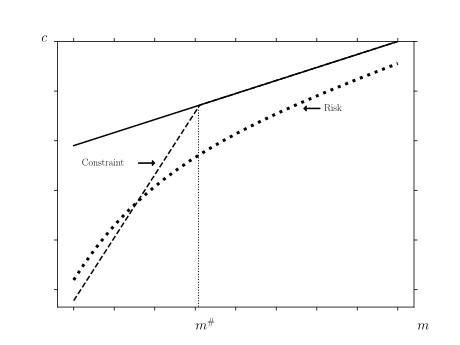
\includegraphics[width=.95\textwidth]{\FigDir/CounterclockwiseConcavifications}}
    \caption{Examples of Counterclockwise Concavifications}
    {\footnotesize \begin{singlespace} {\emph{Notes:} The solid line shows the linear consumption function in the case with no constraints and no risks. The two dashed lines show the consumption function when we introduce a constraint and a risk, respectively. The introduction of a constraint is a counterclockwise concavification of the solid consumption function around ${m}^{\#}$, while the introduction of a risk is a counterclockwise concavification around $\infty$.}  \end{singlespace}}
    \label{fig:counterclockwise}
  \end{figure}

  \noindent Figure \ref{fig:counterclockwise} illustrates two examples of counterclockwise concavifications: the introduction of a constraint or a risk. In both cases, we start from the situation with no risk or constraints (solid line). The constraint causes a counterclockwise concavification around a kink point ${m}^{\#}$. Below ${m}^{\#}$, consumption is lower and the MPC is greater. The introduction of a risk also generates a counterclockwise concavification of the original consumption function, but this time around $\infty$ as described in Lemma \ref{lem:ccrisk}. % For ${m} < \infty$, consumption is lower, the MPC is higher, and the consumption function is strictly more concave than in the original situation (solid line).




  \subsection{A Counterclockwise Concavification Increases Prudence}\label{sec:CCPrud}
  The section above defined a counterclockwise concavification which describes the effects of either a constraint or a risk on consumption concavity. This section shows the relationship between consumption concavity and prudence. Our method is to compare prudence in a \textit{baseline} case where the consumption function is $c({m})$ to prudence in a \textit{modified} situation in which the consumption function $\hat{c}({m})$ is a counterclockwise concavification of the baseline consumption function.

  The first result relates to the effects of a counterclockwise concavification on the absolute prudence of the value function, $-\frac{V'''({m})}{V''({m})}$.


  \begin{lemma}\label{lem:CCToPrud}  (A Counterclockwise Concavification Increases Prudence.) \\
    Consider an agent who has a utility function %of the HARA class \eqref{eq:HARA}
    with $u' > 0$, $u'' < 0$, $u''' \geq 0$, and non-increasing absolute prudence ($-u'''/u''$). If $c({m})$ is concave and $\hat{c}({m})$ is a counterclockwise concavification of $c({m})$, then the value function associated with $\hat{c}({m})$ exhibits greater absolute prudence than the value function associated with $c({m})$ for all ${m}$.
  \end{lemma}

  \noindent See Appendix \ref{app:CCToPrud} for the proof. To understand the effects on prudence of a counterclockwise concavification, note that for a twice differentiable consumption function and thrice differentiable utility function, absolute prudence of the value function is defined as
  \begin{equation} -\frac{V'''({m})}{V''({m})} = - \frac{u'''(c({m}))}{u''(c({m}))}c'({m}) - \frac{c''({m})}{c'({m})} \label{eq:prudence}\end{equation}
  by the envelope condition. The results in Lemma \ref{lem:CCToPrud} follow directly. Lemma \ref{lem:CCToPrud} additionally handles cases where the consumption function is not necessarily twice differentiable.

  There are three channels through which a counterclockwise concavification heightens prudence. First, the increase in consumption concavity from the counterclockwise concavification itself heightens prudence. Second, if the absolute prudence of the utility function is non-increasing, then the reduction in consumption (for some states) from the counterclockwise concavification heightens prudence (at those states). And third, the higher marginal propensity to consume (MPC) from the counterclockwise concavification means that any given variation in market resources results in larger variation in consumption, increasing prudence. The channels operate separately, implying that a counterclockwise concavification heightens prudence \textit{even if absolute prudence is zero} as in the quadratic case.\footnote{cf.\ Nishiyama (\citeyear{nishiyama2012concavity})}

  Lemma \ref{lem:CCToPrud} only provides conditions for when the value function exhibits greater prudence, but not \textit{strictly} greater prudence. In particular, the value function associated with $\hat{c}({m})$ will in some cases (e.g., quadratic utility) have equal prudence most ${m}$ and strictly greater prudence only for some ${m}$. In Lemma \ref{lem:ccandstrictprud}, we provide conditions for when the value function has strictly greater prudence.

  \begin{lemma} \label{lem:ccandstrictprud}(A Counterclockwise Concavification Strictly Increases Prudence.)\\
    Consider an agent who has a utility function with $u' > 0$, $u'' < 0$, $u''' \geq 0$, and non-increasing absolute prudence ($-u'''/u''$). If $c({m})$ is concave and $\hat{c}({m})$ is a counterclockwise concavification of $c({m})$ around ${m}^{\#}$, then the value function associated with $\hat{c}({m})$ exhibits strictly greater prudence than the value function associated with $c({m})$ if the utility function satisfies $u''' > 0$ and ${m} < {m}^{\#}$ or the utility function is quadratic ($u''' = 0$) and $\frac{\hat{c}'({m})}{c'({m})}$ strictly declines at ${m}$.
  \end{lemma}
  \noindent See Appendix \ref{app:ccandstrictprud} for the proof. For prudent consumers ($u''' > 0$), the value function exhibits strictly greater prudence for all $m$ where the counterclockwise concavification affects consumption. This is because a reduction in consumption and higher marginal propensity to consume heighten prudence if the utility function has a positive third derivative and prudence is non-increasing. If the utility function instead is quadratic, the third derivative is zero and absolute prudence of the value function does not depend on the level of consumption or the marginal propensity to consume. In this case, the counterclockwise concavification only affects prudence at the kink points in the consumption function (where $\frac{\hat{c}'({m})}{c'({m})}$ strictly declines at ${m}$).

  We have now defined consumption concavity and the operation called a counterclockwise concavification. In particular, we have shown that a counterclockwise concavification heightens prudence, which is related the precautionary saving. The next section shows how the introduction of a liquidity constraint is a counterclockwise concavification before we use the tools derived in this section to provide the link between liquidity constraints and precautionary saving in Section \ref{sec:LCandPS}.



